\section{Results}
\peng{
Here are some turning parameters that I can think of:
\begin{itemize}
    \item Training data size $M$,
    \item The ratio $\alpha$ of divergence free data sets in $M$, 
    \item The learning rate $\lambda$,
    \item The ConvNet structure.
\end{itemize}


}

\justin{
Some issues we may wish to present:
\begin{itemize}
    \item The success rate on the entire test set for cases of enriched and not enriched test data.
    \item How well the softmax scores distinguish between div and non div. Discuss how the training set size doesn't appear in the success rate, but does have a major effect on how well the softmax scores separate.
    \item Even though the accuracy of our classifier is quite high on the overall test set, we wanted to know how the score the neural net gave for individual vector fields changed as a function of the training data. One could think of this as how confident the network becomes in its classifications as it is trained with more data. In figure BLAH we have 
    
\end{itemize}


\begin{figure}[ht]
		\begin{center}
			\begin{tabular}{cc}
				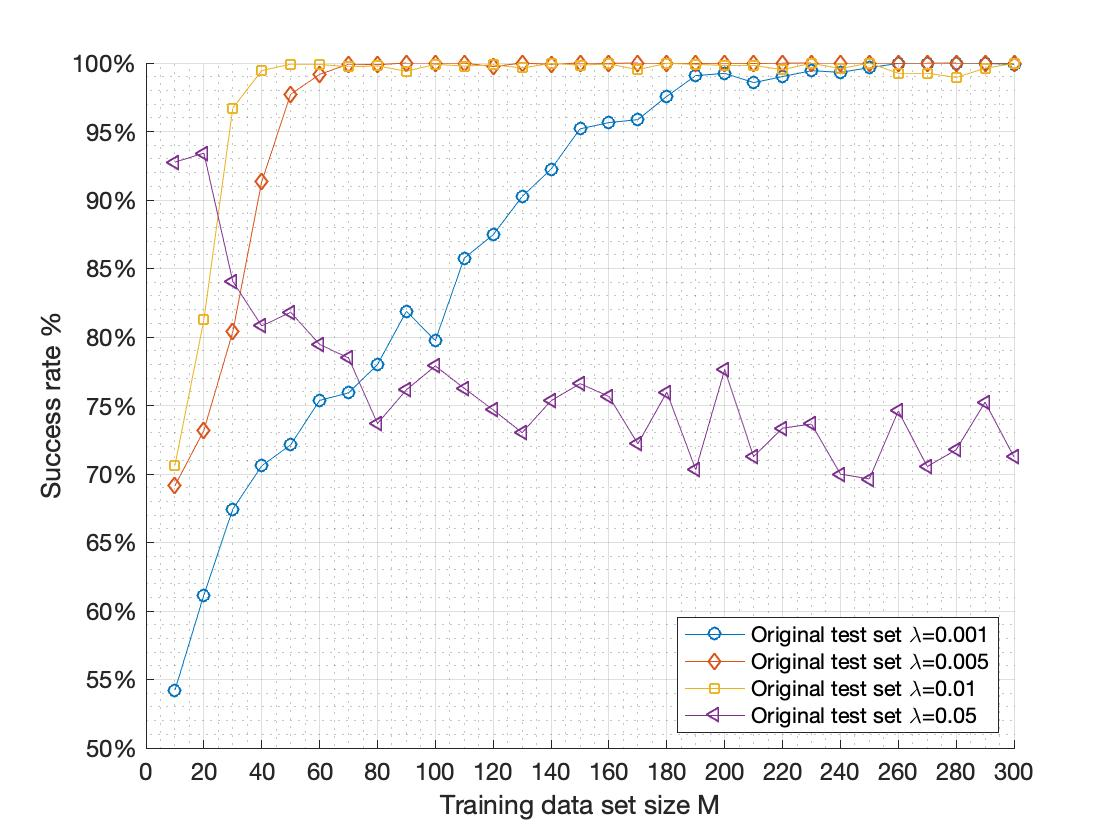
\includegraphics[scale=.15]{orig_sr.jpg}&
				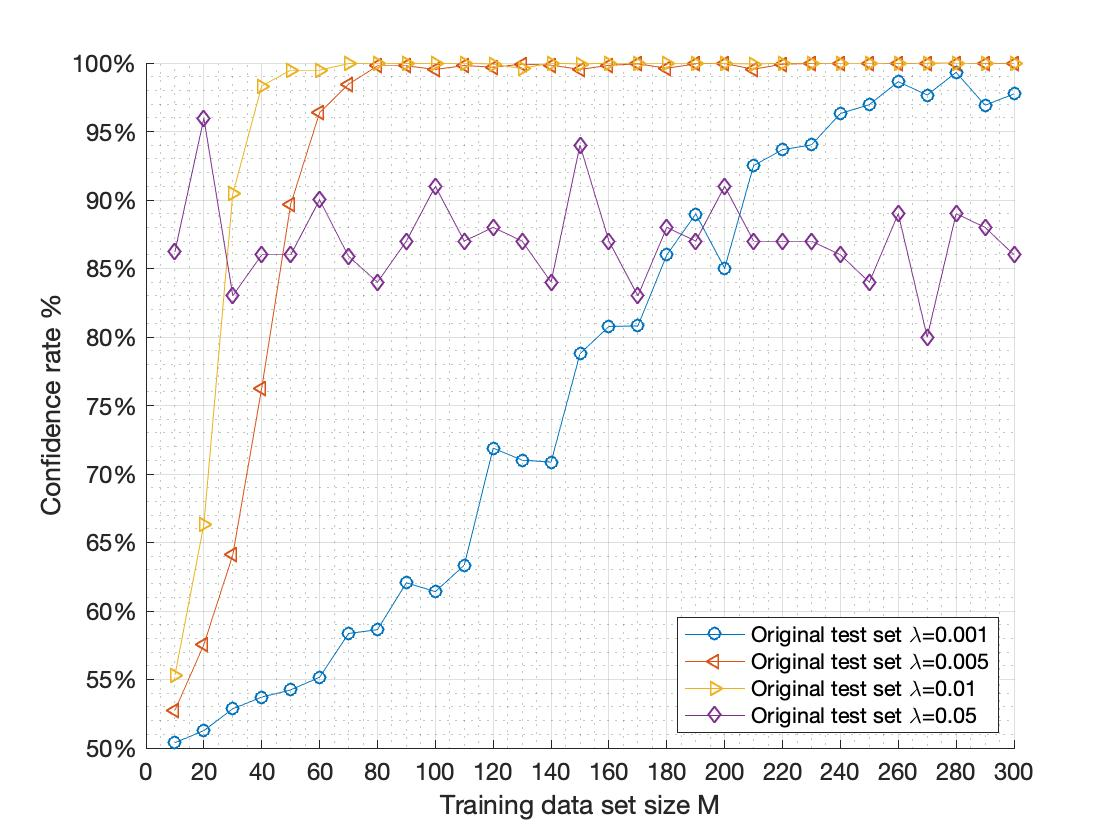
\includegraphics[scale=.15]{orig_cr.jpg} \\
				(a) & (b)
			\end{tabular}
		\end{center}
		\caption{Testing results on original set. 
		(a) The success rate
		(b) The confidence rate on identifying a specific vector field.
		}
		\label{fig:orig_results}
\end{figure}

}